% templates/collated_presentation.tex
\documentclass{beamer}
\usetheme[progressbar=frametitle,block=fill]{metropolis}

\usepackage[english]{babel}  % English language support
\usepackage{microtype}
\usepackage{float}
\usepackage{graphicx} % To include images
\usepackage{booktabs} % For better table rules
\usepackage{textcomp} % For symbols like \textperthousand

\metroset{block=fill}

\title{LLM Sentiment Analysis on AWS Lambda} % Title
\subtitle{Cloud Computing --- Project Presentation} % Subtitle
\author{Dario Loi, 1940849 \and Francesco Fazzari, 1935070} % Authors
\institute{Sapienza, University of Rome} % Institute
\date{\today}

\def\bibfont{\tiny}

\begin{document}

\begin{frame}
\titlepage%
\end{frame}


\section{Introduction}
\begin{frame}{The Goal}
    To deploy a sentiment analysis classifier on a serverless architecture and evaluate its real-time performance on CPU-only infrastructure. The model analyzes emotional tone in text, classifying it as happy, angry, sad, or other.
\end{frame}

\begin{frame}{The Method}
    We leveraged AWS Lambda for its auto-scaling and simplicity. To overcome the challenges of large model sizes and dependencies, we used advanced techniques like model quantization and compilation to the ONNX standard.
\end{frame}

\begin{frame}{The Evaluation}
    An extensive benchmark was performed using the Locust testing framework to simulate realistic user loads. We measured both user-oriented (e.g., response time) and system-oriented (e.g., concurrency) metrics.
\end{frame}

\section{System Architecture \& Optimization}
\begin{frame}{System Architecture}
    \begin{figure}[H]
        \centering
        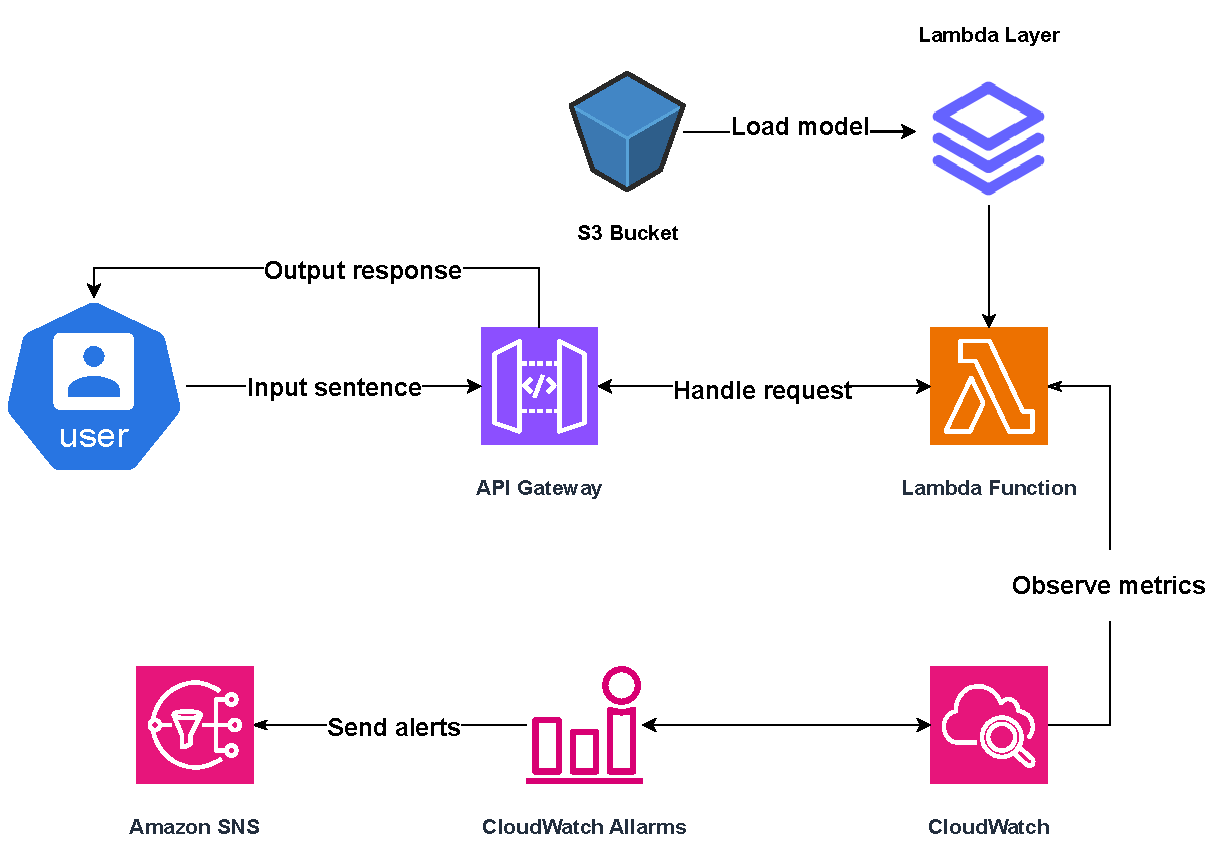
\includegraphics[width=0.7\textwidth]{emo-diag.pdf}
        \caption{The user sends a sentence to an API Gateway, which triggers an AWS Lambda function. The function loads an optimized AI model from an S3 bucket to perform inference. Metrics are monitored by CloudWatch, which sends alerts via Amazon SNS if issues are detected.}
    \end{figure}
\end{frame}

\begin{frame}{AI Model Optimization}
    \begin{alertblock}{The Challenge}
        Deploying large AI models on serverless platforms like AWS Lambda presents two main hurdles:
        \begin{itemize}
            \item The PyTorch framework is too large, exceeding AWS Lambda's size limits.
            \item The model's parameters are in the dozens of megabytes, also violating size constraints.
        \end{itemize}
    \end{alertblock}
\end{frame}

\begin{frame}{AI Model Optimization}
    \begin{exampleblock}{The Solution: Quantization}
        \begin{itemize}
            \item We converted our MobileBERT model to the \textbf{ONNX standard}, allowing us to use the much lighter \texttt{onnxruntime} library.
            \item During conversion, we performed \textbf{dynamic quantization}, reducing the model's parameters from 32-bit floats to 8-bit unsigned integers.
            \item \textbf{Result:} Model size was reduced by a factor of $\approx3.68$, from 81.5 MiB to just 22.1 MiB.
        \end{itemize}
    \end{exampleblock}
\end{frame}


\section{Performance Evaluation}
\begin{frame}{Load Testing Scenarios}
    We used Locust to simulate realistic user behavior under three distinct scenarios to test horizontal scaling and robustness.
    
    \begin{table}[H]
        \centering
        \caption{Load Testing Configurations }
        \begin{tabular}{lcccc}
            \toprule
            \textbf{Scenario} & \textbf{Users} & \textbf{Ramp-up} & \textbf{Duration} & \textbf{Request Delay (s)} \\
            \midrule
            Bursty & 3 & 3 s & 2 min & [5, 10] \\
            Medium & 50 & 25 s & 2 min & [3, 5] \\
            Heavy & 100 & 50 s & 1 min & [1, 3] \\
            \bottomrule
        \end{tabular}
    \end{table}
    
    \vspace{1em}
    
    \begin{itemize}
        \item \textbf{Bursty:} Models sparse, intermittent requests.
        \item \textbf{Medium \& Heavy:} Test the infrastructure's ability to handle significant and high volumes of traffic.
    \end{itemize}
\end{frame}

\section{Results}
\begin{frame}{Results: Concurrency and Scaling}
    \begin{figure}[H]
        \centering
        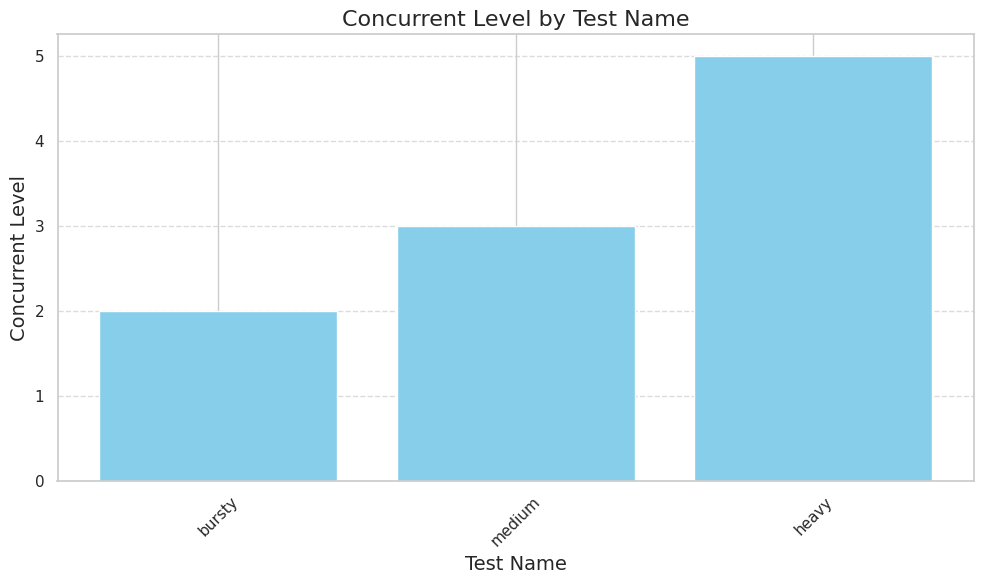
\includegraphics[width=0.7\textwidth]{conc_levels.png}
        \caption{Maximum concurrent Lambda executions as reported by CloudWatch during each test.}
    \end{figure}
\end{frame}

\begin{frame}{Results: Concurrency and Scaling}
    \begin{block}{Insight}
        The system is incredibly efficient. Even under a ``Heavy'' load of 100 concurrent users, the infrastructure scaled to a maximum of only \textbf{5 concurrent Lambda instances}. This demonstrates excellent horizontal scaling and cost-effectiveness, processing thousands of requests with 100\% availability.
    \end{block}
\end{frame}

\begin{frame}{Results: Horizontal Scaling Under Load}
    \begin{figure}[H]
        \centering
        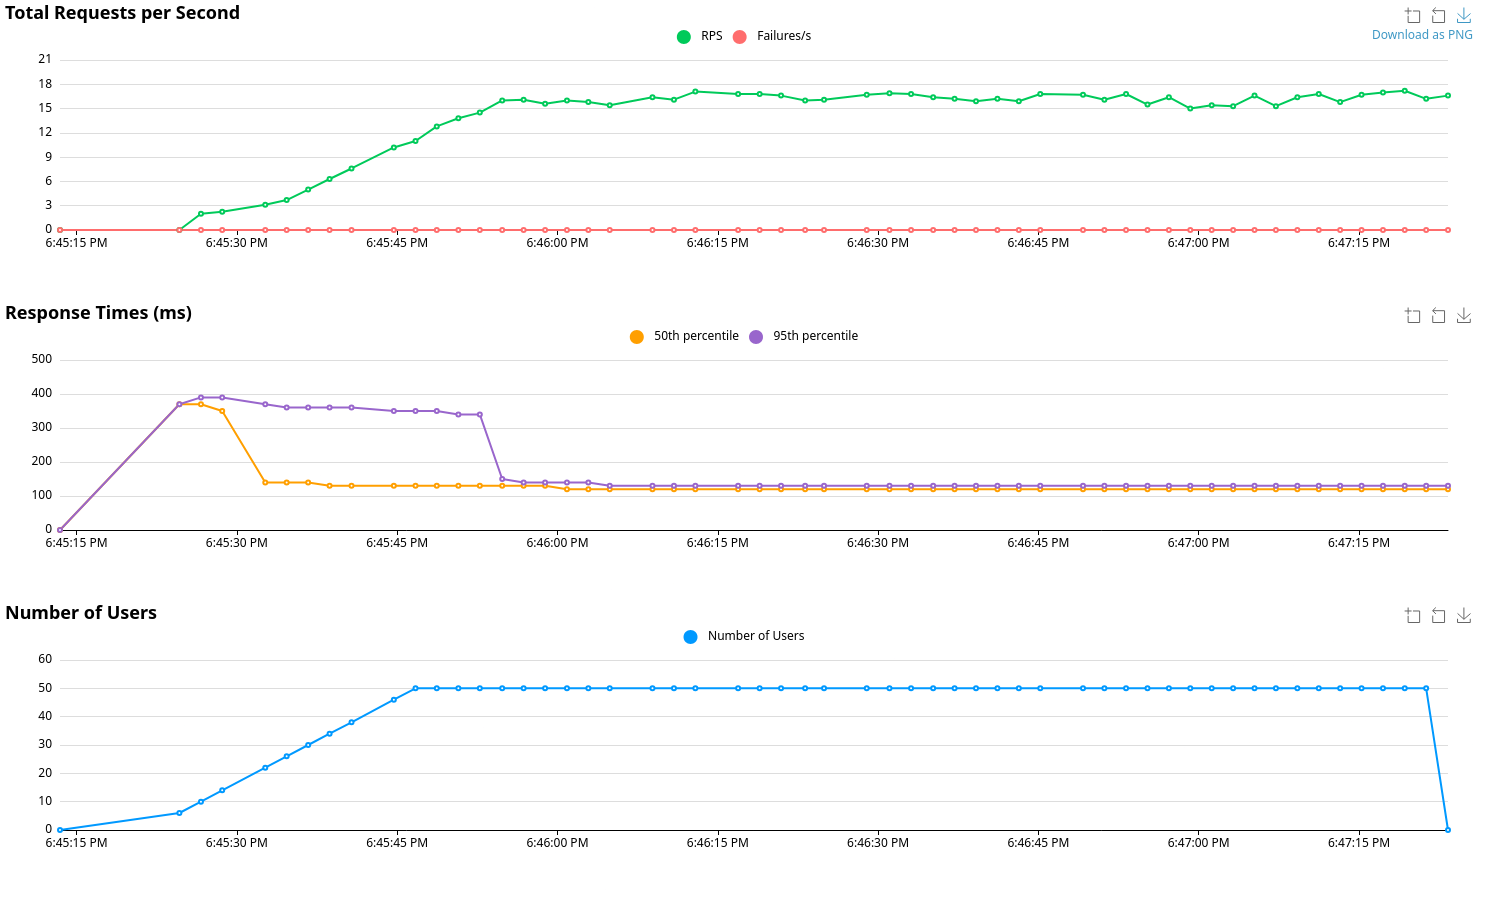
\includegraphics[width=\textwidth]{medium_load_test.png}
        \caption{Graphs for the Medium Load Test.}
    \end{figure}
\end{frame}

\begin{frame}{Results: Horizontal Scaling Under Load}
    \begin{block}{Insight}
        The top graph shows a linear correlation between active users and requests per second, indicating successful scaling. The high 99th-percentile response time during the ramp-up period (middle graph) suggests that new users were assigned to new Lambda instances, forcing a ``cold start'' and proving that our infrastructure was \textbf{actively and automatically scaling out} to meet demand.
    \end{block}
\end{frame}

\begin{frame}{Results: Vertical Scaling}
    \begin{figure}[H]
        \centering
        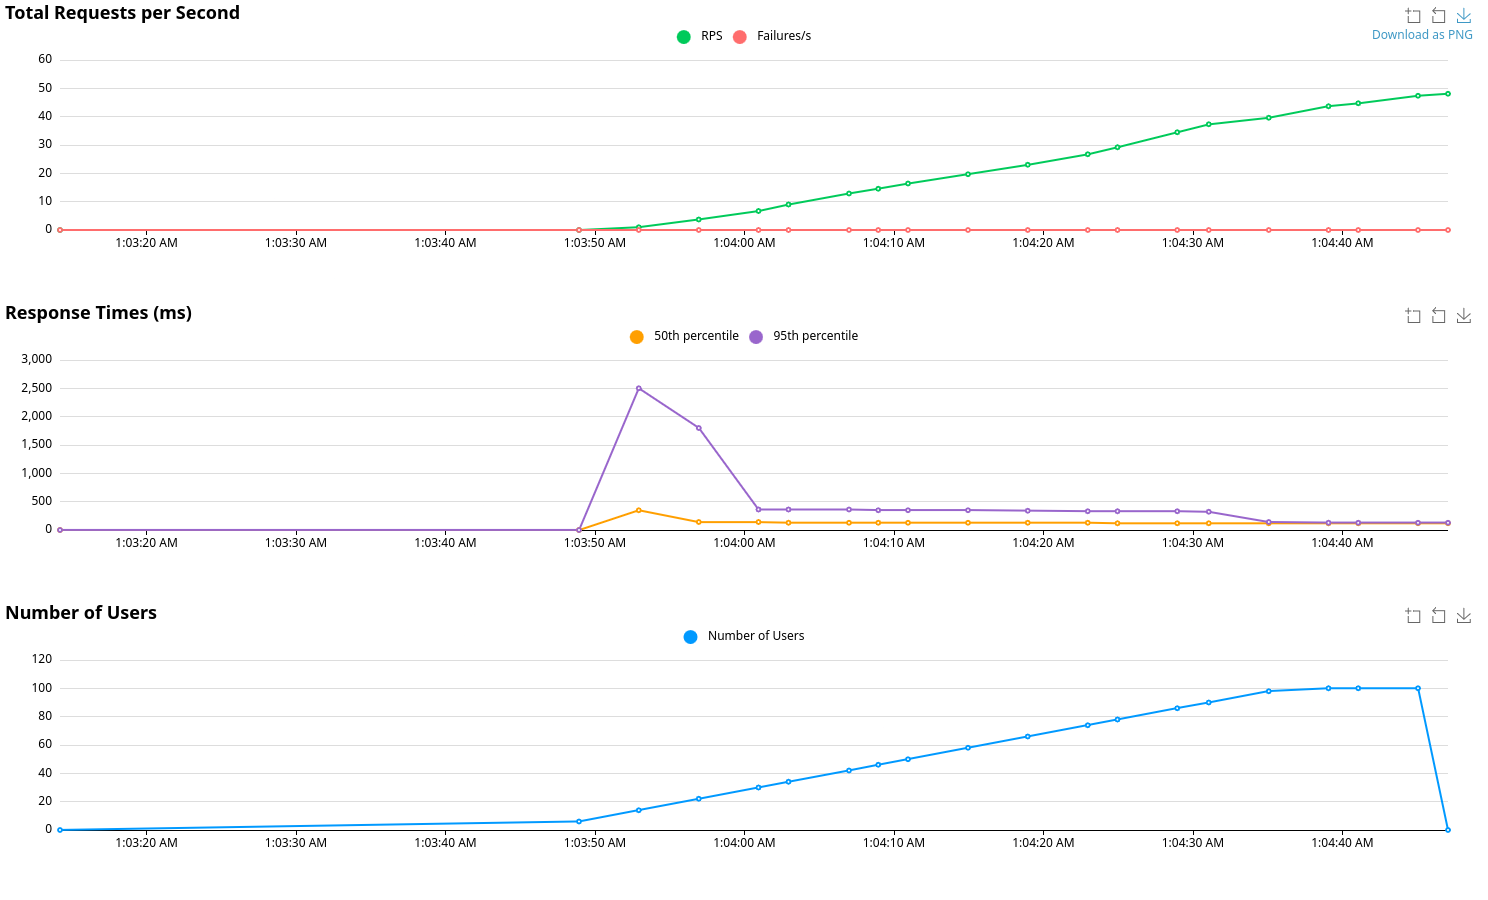
\includegraphics[width=0.9\textwidth]{heavy_scale_graphs.png}
        \caption{Graphs for the Heavy Load Test with Lambda RAM doubled to 1024 MiB.}
    \end{figure}
\end{frame}

\begin{frame}{Results: Vertical Scaling}
    \begin{block}{Insight}
        Doubling the provisioned RAM (and associated CPU power) showed \textbf{no significant improvement} in response times. This suggests that individual requests were already being processed near-optimally and that the primary bottleneck is not compute resources, but rather network overhead, which we estimated to be around 100ms.
    \end{block}
\end{frame}

\begin{frame}{Aggregated Performance}
    \begin{alertblock}{Key Takeaway}
        Across all three demanding test scenarios, the service handled thousands of requests with \textbf{zero failures or errors}. The median response time remained stable at around 120-130ms, demonstrating a robust and reliable system. The high ``Max'' times are attributed to initial ``cold starts''.
    \end{alertblock}
\end{frame}

\section{Conclusion}
\begin{frame}{Conclusion}
    \begin{block}{Achievements}
        \begin{itemize}
            \item We successfully demonstrated that it's possible to deploy a lightweight, efficient, and performant LLM for a real-world task on a serverless, CPU-only cloud architecture.
            \item Our proposed architecture proved to be simple, highly scalable, and fault-free under realistic traffic loads.
        \end{itemize}
    \end{block}
\end{frame}

\begin{frame}{Conclusion}
    \begin{alertblock}{Key Findings}
        \begin{itemize}
            \item The system scales effortlessly to meet user demand, both horizontally (adding instances) and vertically (utilizing resources).
            \item The primary performance bottleneck was identified as network overhead, not computational power.
        \end{itemize}
    \end{alertblock}
    \begin{exampleblock}{Future Work}
        Network latency could be further reduced by deploying the serverless infrastructure closer to end-users via edge locations, an easy-to-implement next step.
    \end{exampleblock}
\end{frame}


\begin{frame}{The End}
    \begin{center}
        \Huge Thank you for your attention!\\
        Questions?
    \end{center}
\end{frame}



\end{document}
